%
% 1
%
\chapter{Introduction}%
	%
	%
	\label{ch:introduction}
	\index{Course!Introduction}%
	%
  %
  \begin{mybox}%
  \footnotesize{%
  \newthought{Dear reader,}\\[1em]%
	%
	\newthought{You probably find yourself reading this} because you enrolled in Statistical Reasoning and Quantitative Methods (\SRQM), a postgraduate introduction to statistics that Ivaylo Petev and myself have been teaching at Sciences~Po in Paris since 2010.%
  
  \newthought{This guide} is a practical handbook to read while taking the course. The rest of the teaching material, which includes the syllabus and essential files to be used in and outside class, can be downloaded from the course webpage at the following address:\\[1em]%

    \url{http://f.briatte.org/teaching/quanti/}\\[1em]%
		
  \newthought{Start reading below} to learn about the course basics, making sure in particular that you have \textbf{run the course setup} on your computer and that you know how to run it again if necessary. Welcome to the course!%

  }%
  \end{mybox}
  %
  %
  % \minitoc
  \startcontents[chapters]%
  \printcontents[chapters]{l}{1}{\setcounter{tocdepth}{2}}%
	%
	\newpage
	%
	%

%
% 1.1
%
%
% 1.1
%
% \section{Topics}%
%   %
%   %
%   \label{sec:topic}%
	\index{Methods}%
	%
	%

% 1.1.1
%
% \subsection{Quantitative methods}
%   %
%   %
	\label{sec:quantitative-methods}
  \index{Quantitative methods}%
  
	\newthought{Quantitative methods} designate a branch of social science methodology that applies statistical procedures to experimental or observational data in order to produce explanatory models for the complex, recurrent phenomena that affect populations and organizations. These methods can be used to analyze things like attitudes towards highly skilled and low-skilled immigration in the United States,\footcite{HainmuellerHiscox:2010a} the effects of a program to develop fertilizer use in Kenya,\footcite{DufloKremer:2009a} or the historical vote that put Adolf Hitler into power in interwar Germany.\footcite{KingRosen:2008a}%
		%
		%

	The models produced by quantitative research account for the regularities that exist in the data by estimating how a set of independent, explanatory variables can predict the value of a dependent, outcome variable. To what extent, for example, is the prevalence of HIV/AIDS predictable from the level of economic inequality and degree of political unrest in a country? Does the support for violent action vary with age and education, in what direction, by how much, within what range and at what rate? A quantitative model can estimate these relationships, on top of which researchers develop theories to explain what causal paths are followed in the model.%
		%
		%

	A strong background assumption behind such questions is comparability. In quantitative data, the units of observation, such as individuals or countries, are defined through a set of commensurable characteristics—the variables. The first and perhaps most important requirement of a quantitative model is that you are measuring roughly the same thing among roughly similar units with sufficient reliability. This is far from obvious when you are aggregating, for instance, development statistics, because many countries have very low statistical capacity (among many other issues).\footcite{Jerven:2013a}%
		%
		%

	Each variable of a quantitative model is then attached to a concept, like `household income' or `democratic status,' each of which provides an explanatory component for the dependent variable. Measuring the predictive effect of the `independent' variables onto the `dependent' one is therefore a means to measure the respective influence of each explanatory component onto a given phenomenon, which might be a measure of something, like the number of children in a household or the GDP growth rate of a country, or the probability of occurence of something, like abortion or state collapse.%
		%
		%

	\newthought{From a learning perspective,} what you can immediately figure out of the short description above is that quantitative methods require some attention to terminology: `data' are `observations' described by `variables' made of `values', some of which we `predict' from the others through the `estimation' of their `independent' effects. The topic also requires some (really light) exposure to logic and mathematics. Finally, any quantitative analysis requires some knowledge of the practical aspects of empirical research design, such as data collection or sampling.%
		%
		%

	Contrary to what bookshelves of statistics textbooks and horror stories about equations feeding on human flesh might have led you to believe, your learning approach of quantitative analysis should actually have much more to do with its practice than with its theory. The practice of quantitative data analysis implies, for example, that you have to try things out until `they work' at the technical level. This aspect of things requires a lot of independent learning through trial-and-error.%
		%
		%
	
	Another practical dimension of quantitative analysis in the social sciences has to do with the limited degree of precision of any social statistic, which makes issues of statistical significance secondary to issues of measurement accuracy and data availability when it comes to social data. When your unit of analysis is a social one, start thinking in rounded figures: the measures are never more precise than what they are, nor the data more representative than what it can possibly be.%
		%
		\footnote{For that matter, a report that would speak of `1.474\% of the general population' is almost never going to be a credible result with social data, because three-digit precision would indicate spectacularly precise estimation.}%
		%
		%


% 1.1.2
%
% \subsection{About this guide}%
%   %
%   %
	\newthought{This `Stata guide'} was written as an introduction to Stata for students with a background in the social sciences. You are not expected to know anything about statistics, but you are expected to know a few things about social science research from your undergraduate curriculum. You should be familiar, for instance, with notions like cultural capital, gross domestic product per capita and political regimes.%
		%
		%

	We will cover the following topics:%

	\begin{itemize}
		\item This introduction deals with the course basics, essential computer skills and Stata fundamentals. It also explains how to set up a computer for the course.%
	
		\item %
		Section~\ref{ch:data} explains how to prepare data for analysis, and %
		Section~\ref{ch:distr} explains how to visualize distributions. This segment is primarily about description and univariate statistics. %
    It ends on instructions to submit your first draft.
	
		\item %
		Section~\ref{ch:asso} introduces statistical significance tests, and %
		Section~\ref{ch:ols} introduces ordinary least squares and simple linear regression. This segment is about association and bivariate statistics. %
    It ends on instructions to submit your revised draft.

		\item %
		Section~\ref{ch:lin} introduces multiple linear regression modelling, and %
		Section~\ref{ch:log} introduces logistic regression modelling. This segment covers the basics of statistical modelling for continuous and categorical variables in cross-sectional data. %

    The guide also includes an index including all commands cited in the text, and a list of bibliographic references.%
	\end{itemize}

\newthought{Several sections of the guide are still in draft form}, so watch for updates and read it along other documentation. Its writing started with students questions, and several sections were first written as short tutorials concerning specific issues with data management. One thing led to another, and we ended up with the current document. The aim is to cover 90\% of the course by version 1.0.%

	Several students have already provided very valuable feedback on the text—thanks, and keep the feedback flowing in!%

%
%
% 1.2
%
%
% 1.2
%
\section{Course setup}%
	%
	%
	\label{sec:course-setup}%
	\index{Course!Setup}%
	%
	%
	
	\newthought{This course uses Stata} as its statistical software of choice. Stata is used by many social scientists working with quantitative data in areas such as economics and political science.%
	%
 	\footnote{For example, you will find Stata output in some of Nate Silver's work at the \emph{New York Times} on his `FiveThirtyEight' electoral blog; see, \eg, ``'\href{http://fivethirtyeight.blogs.nytimes.com/2012/03/12/polling-in-deep-south-has-posed-challenges/}{Polling in Deep South Has Posed Challenges},'' 12 March 2012.} %
	%
	Most statistical procedures used in these disciplines know some form of implementation in Stata, and the software is supported by a large user community. It provides a good middle ground between a spreadsheet editor and a statistical programming environment.%
  	
	\newthought{This section} explains how to set up Stata to follow the course. It assumes very little knowledge of computers. \hlred{\textbf{Make sure that you successfully set up your computer} for the course, and that you know how to run the setup again if needed.}%

  \newthought{We will use the `Standard Edition'} (\textsc{se}) of Stata~12 that works on most current computers.%
  \footnote{See the list of Stata products and compatible operating systems: %
		\url{http://www.stata.com/products/compatible-operating-systems/}}%
		%
		The keyboard shortcuts we provide are for \OSX (Mac) and Windows (Win). The installation procedures on both systems are almost identical:% 
		
	\begin{description}

		\item[On \OSX] %
		%
		The entire Stata application folder should be located in the \texttt{Applications} folder. You should drag the Stata application icon to your Dock for quicker access. The \kbd{Cmd} (Command) key used in keyboard shortcuts is the `Apple' modifier key located left and right of the spacebar.%

		\item[On Windows] %
		%
		The entire Stata application folder should be located in the \texttt{Program Files} folder, or whatever your version of Windows calls it. You should drag the Stata application icon to your Taskbar for quicker access. The \kbd{Ctrl} key used in keyboard shortcuts is the `Control' modifier key located bottom-left of the spacebar.%

	\end{description}

	The course runs fine on older versions of Stata. The setup below has been tested on Sciences Po workstations equipped with Stata~11.%
	
	% 0.2.1
	%
	\subsection{Get the teaching material}%
		\label{sec:teaching-pack}%
		\index{Course!Teaching material}

	\newthought{The `Teaching Pack' for this course comes in a single folder,} called the \SRQM folder, which you will have to access very frequently inside and outside class. Download and unzip the folder from its webpage%
		\footnote{\url{http://f.briatte.org/srqm/}} %
		or use the copy provided in class, and keep the \ZIP archive of the folder as a backup.%
		
	\hlred{Move the \SRQM folder to a \textbf{stable location} that you can easily locate on your hard drive, and keep it at that same location throughout the entire course.} Most users deal with this requirement by putting the \SRQM folder with the rest of their study files and then creating an alias to it on their Desktop.%
	
	Use any method that does not involve clicking for two full minutes to access the \SRQM folder, and do not rename its enclosing folders. For simplicity, leave the folder name to \SRQM for the class, and rename it to whatever you like at the end of the semester.%
	
	At that stage, \textbf{check the contents} of the \SRQM folder. The \SRQM folder contains the entire course material, minus the copyrighted textbooks and Stata software. The full contents of that folder, shown in Figure~\ref{fig:srqm-folder}, must stay available on your hard drive during the entire course.%
		%
		%

		\begin{figure}%
		  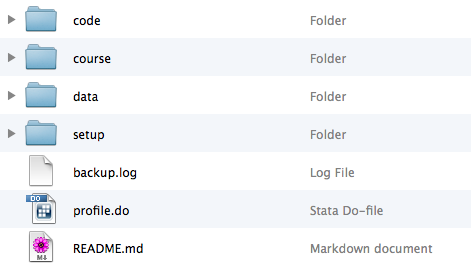
\includegraphics[width=\textwidth]{srqm-folder}
      
		  \caption{The contents of the \SRQM folder should match %
			this screenshot from a \OSX setup.}
		  \label{fig:srqm-folder}
		\end{figure}
		%
		%
		
	The \course folder contains the course slides and syllabus, as well as this guide. The \data folder contains a selection teaching datasets, and the \code folder will host the course do-files (covered below at p.~\pageref{sec:do-files}). The \setup folder and \texttt{profile.do} files provide additional course functionalities. All folders are required for the course to roll out properly.%
		%
		%	\index{Computers!File and folder paths}%

	\index{Computers!URLs}%
	You need to understand the file structure of the course to understand how Stata will locate its files and folders from their \textbf{paths}. The path to the \SRQM folder, for example, might look like this on \OSX:\\[1em]%
	
	\begin{docspec}
		/Users/fr/Documents/Teaching/SRQM
	\end{docspec}
	
	On Windows, the path generally starts on the \texttt{C:} drive and is shown with \texttt{\textbackslash} backslashes:%
		\footnote{Stata for Windows also understand paths with forward slashes.}%
    
	\begin{docspec}
		C:\textbackslash{}Users\textbackslash{}Ivo\textbackslash{}Desktop\textbackslash{}SRQM
	\end{docspec}
	
	Once a folder has been set as the \emph{working directory}, Stata can locate files and folders from within it by using relative paths. The example below shows the relative path of the \texttt{nhis2009.dta} dataset in the \texttt{\data} folder:\\[1em]%
	
	\begin{docspec}
		/Users/fr/Documents/Teaching/SRQM/\hlred{\underline{data/nhis2009.dta}}
	\end{docspec}

	File paths are used in Stata to open and save datasets and other types of files. In some cases, it is also possible to open files from online sources by specifying their \URL. A \URL is an Internet address like the one that brings up the course webpage.%
		\footnote{\url{http://f.briatte.org/teaching/quanti/}}%
		%
		%
	
	We will use file paths and URLs extensively throughout the course, so make sure that you understand both. I do my best to keep things tidy on my end by using Internet shortlinks and simple, informative folder and file names for the course material. You will have to do the same on your end.%
		%
		\footnote{For instance, you will be required to submit your work under a specific group name that includes your family names in alphabetical order.}%
		%
		%

	% 0.2.2
	%
	\subsection{Set your working directory}%
		\label{sec:working-directory}%
		\index{Course!Teaching material}

  \newthought{Open the Stata program.} \OSX users can simply double-click the application icon (Figure~\ref{fig:stata-icon}). \hlred{\textbf{Windows users} will have to run Stata with administrator privileges: do this by right-clicking the Stata application icon then selecting `Run as Administrator.'} This will allow Stata to save files anywhere on the hard drive, which is required only for this setup.%

		\begin{marginfigure}
			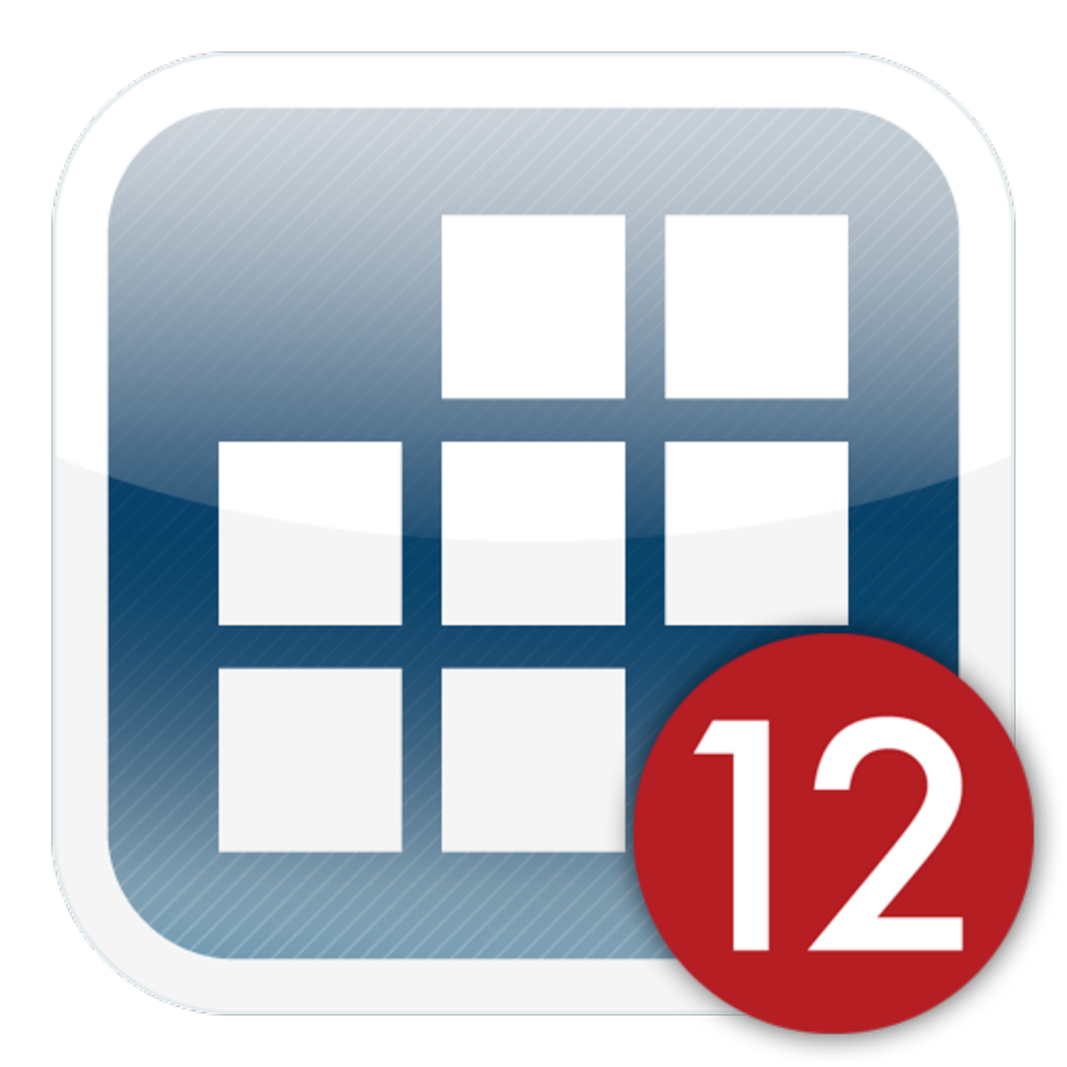
\includegraphics[width=.75\textwidth]{stata-icon}
			\caption{The Stata~12 icon.}
			\label{fig:stata-icon}
	  \end{marginfigure}
	 
	You are now going to set the working directory, which is the folder in which Stata opens and saves files by default. From the `File' menu, choose `Change working directory...', then select the \SRQM folder and press \texttt{Enter}. You will see something like the following printed in the Results window, that is, a folder path ending with the \SRQM folder:\\[1em]%
	
		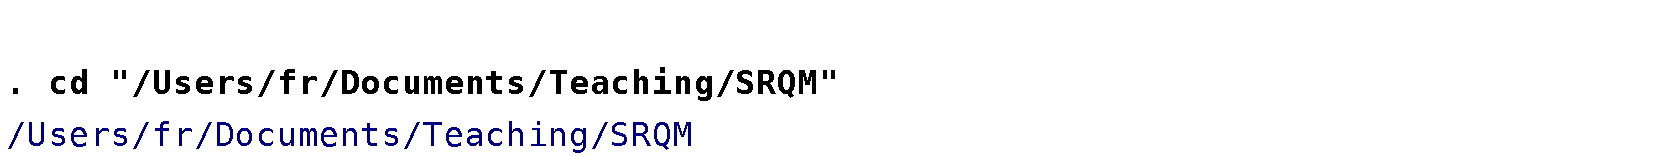
\includegraphics{srqm-cd}\\[1em]

	As the code output shows, the Stata command to do what you did through the `File' menu is \cmd{cd}, for `\underline{c}hoose \underline{d}irectory,' followed by the path to the desired folder. Now that you have learnt a Stata command, try it out by typing the following lines in the Command window and pressing \texttt{Enter} to execute each line:%
	
	\begin{docspec}
		cd ..\\
		cd SRQM
	\end{docspec}
	
	The first command, \texttt{cd ..}, changes the working directory to the enclosing folder, which in my case is the \texttt{Teaching} folder. The second command returns to the \SRQM folder and makes it the working directory again:\\[1em]%
		
	
\includegraphics{srqm-cd-back}\\[1em]
	
	You can also list the contents of the working directory with the \cmd{ls} command. The example below will show the full contents of the \SRQM folder with detailed file information:%
	
		\begin{docspec}
			ls
		\end{docspec}

		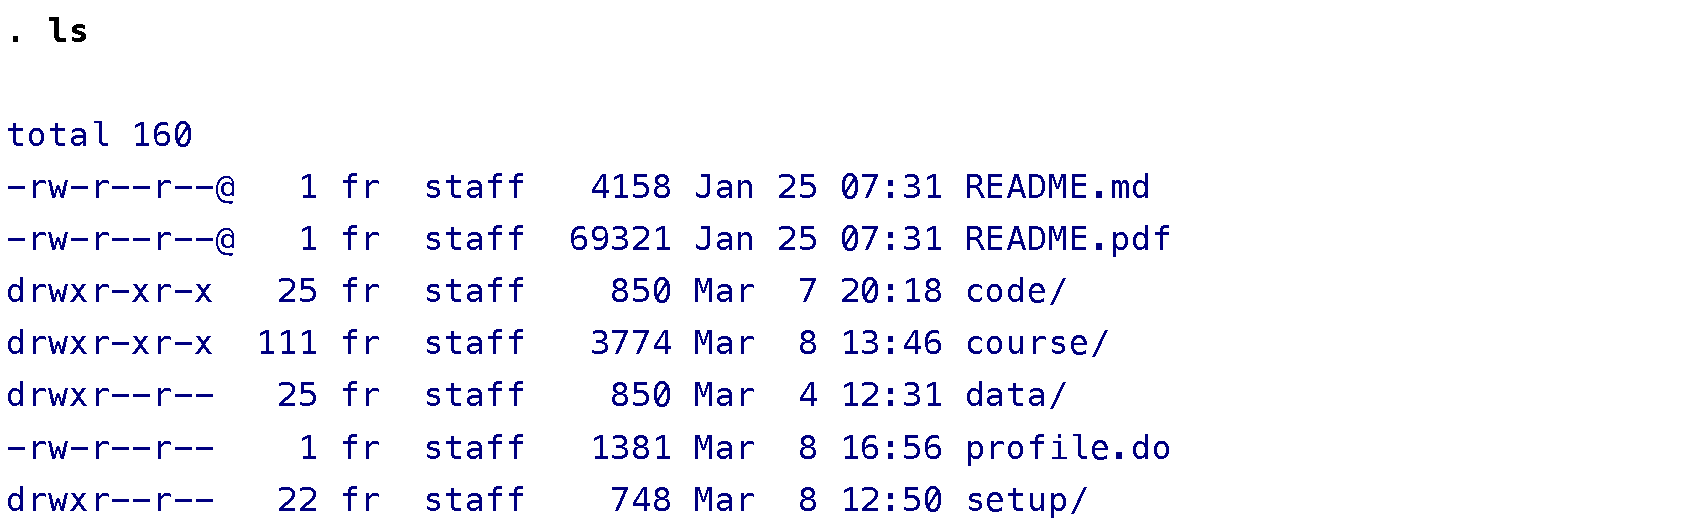
\includegraphics{srqm-ls}\\[1em]
			
	The \cmd{ls} command below will produce a more focused output by listing only the files located in the \data folder that end with the \ext{.dta} extension, which is the Stata dataset format (Figure~\ref{fig:stata-dta}):%

		\begin{marginfigure}
			
\includegraphics[width=.75\textwidth]{stata-dta-icon}
			\caption{Stata~12 dataset icon.}
			\label{fig:stata-dta}
		\end{marginfigure}

		\begin{docspec}
			ls data/*.dta, w
		\end{docspec}
			 
	The command will list the teaching datasets used in the course, for which some documentation is available in the course appendix at p.~\pageref{sec:data-sources}. The \cmd{ls} command is told to only show their filenames by passing the \coab{wide}{w}{ls} option to it:\\[1em]%
 
		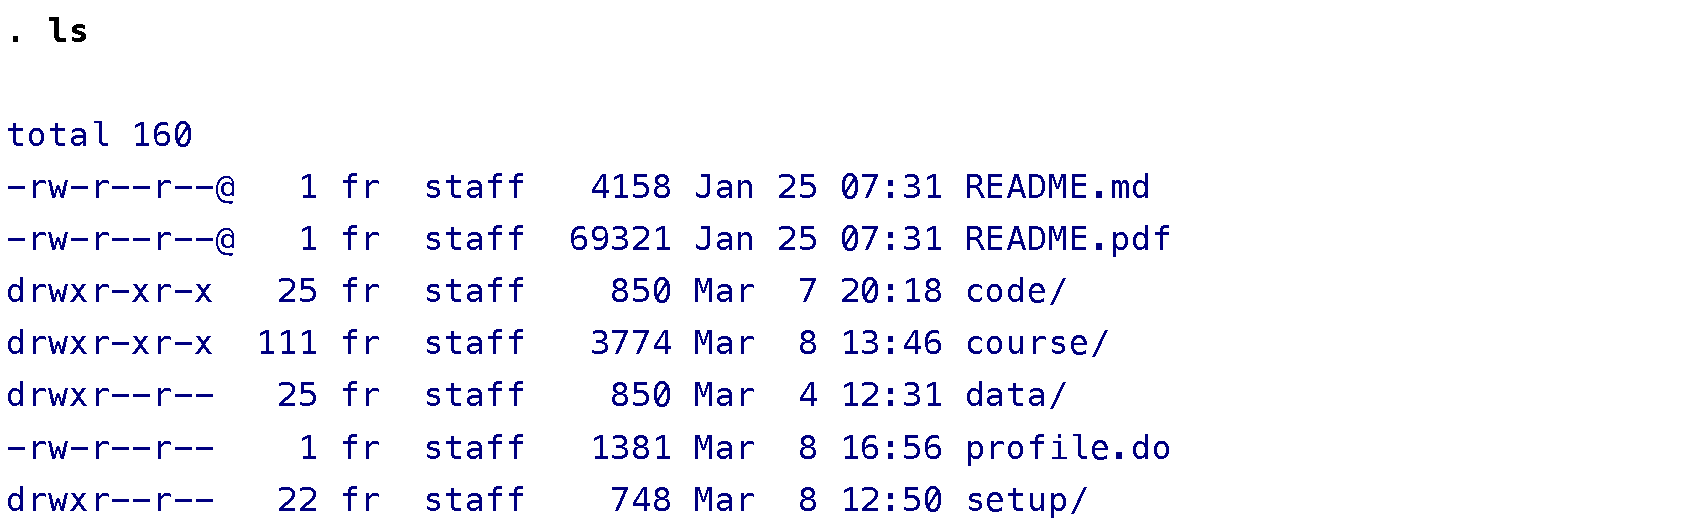
\includegraphics{srqm-ls}\\[1em]
	
	To finish this little exercise with folder navigation from the command line, make sure that your working directory is the \SRQM folder. Use the \cmd{pwd} command to get the path printed once more:%
	
		\begin{docspec}
			pwd
		\end{docspec}
	
	Your working directory should again end with the \SRQM folder, which is what we need to run the course setup in the next section:\\[1em]%
	
		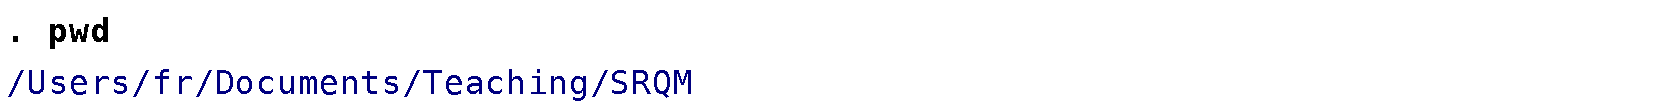
\includegraphics{srqm-pwd}\\[1em]
  
  %
	%
	% 0.2.3
  %
  \subsection{Run the \SRQM setup}%
		\label{sec:setup}%

	To finish setting up your computer for the course, make sure that you are connected to the Internet, then type the following command in the Command window and press \texttt{Enter}:%
		%
		%
		
		\begin{docspec}
			run profile
		\end{docspec}
	
	\hlred{\textbf{Note:} the command will not work if you have not set the \SRQM folder as your working directory}, and that its syntax is a strict one: do not add capital letters, separate the words \texttt{run} and \texttt{profile}, and of course, use the exact spelling.%
	
	This command will trigger a bunch of setup utilities that install the additional Stata commands listed in Table~\ref{tbl:additional-commands}, uncompress the course datasets and adjust some Stata system options.%
		%
		\footnote{For example, the setup adjusts Stata memory on older versions of Stata to deal with some of the larger course datasets. Stata~12 now handles memory automatically.} %
		%
		%
		
	\bigskip
 
  \begin{fullwidth}
		\begin{table}
			\footnotesize
			\begin{tabular}{lll}
			\toprule
			Package & Description \\
			\midrule
			\emph{Installed from the \SSC server:} & & \\
		  \quad \cmd{estout} & export regression results \\
			\quad \cmd{fre} & frequencies with value labels \\
		  \quad \cmd{kountry} & standardised regions and country names\\
		  \quad \cmd{leanout} & simplified regression results\\
			\quad \cmd{lookfor\_all} & search for variables across datasets \\
		  \quad \cmd{mkcorr} & export correlation tables\\
		  \quad \cmd{plotbeta} & regression coefficient plots \\
      \quad \cmd{scheme-burd} & blue-red graph scheme\\
			\quad \cmd{spineplot} & mosaic plots \\
		  \quad \cmd{spmap} & maps\\
		  \quad \cmd{tab\_chi} & residuals for Chi-squared tests\\
		  \quad \cmd{tabout} & export summary statistics\\
		  \quad \cmd{wbopendata} & download World Bank data\\
			\addlinespace
			\emph{Installed from elsewhere:} & & \\
			\quad \label{install-gstd01}\cmd{gstd01} & standardize a variable to $0$-$1$; used at p.~\pageref{sec:gtsd01}\\%
			\quad \label{install-clarify}\cmd{clarify} & simulation\\%; used at p.~\pageref{sec:clarify}\\
			\quad \cmd{schemes} & additional graph schemes\\
			\bottomrule\\[.5em]
			\end{tabular}
			%
			\caption{Additional commands installed by the course setup.}%
			\label{tbl:additional-commands}
		\end{table}
  \end{fullwidth}
  
	You will get a `\texttt{Hello!}' message when the setup is complete.%
	
  \hlred{\textbf{Note:} if you move or rename the \SRQM folder, the setup will break and you will have to repeat the steps covered in the previous paragraphs to fix the issue:}%
		%
		%	
		\begin{enumerate}
			\item run as administrator (if using Windows),
			\item select the \SRQM folder as the working directory, and
			\item type \texttt{run profile} to go through setup again.
		\end{enumerate}
	  
	The setup overwrites the \filename{profile.do} file of the Stata application folder to redirect it to the \SRQM folder for the time of the course. From there, it runs another \filename{profile.do} file that verifies the integrity of the teaching material and reruns parts of the setup if necessary.%
		%
		%
		
	The setup also loads the \cmd{srqm} teaching utilities, like \cmd{srqm\_get}, which is used in class to download the latest version of the course material from a temporary course server, and \cmd{stab}, which is used to produce \underline{s}imple \underline{tab}les of summary statistics (see its detailed instructions at p.~\pageref{cmd:stab}).%
    %
    %
		
  \newthought{At the end of the course}, delete the \texttt{profile.do} from the Stata application folder to stop automatically setting the \SRQM folder as your working directory. Alternately, run the \texttt{srqm\_link, clean} command to do so and get a `\texttt{Bye}' message. This will let you work with Stata from any other working directory.%
		%
		%%
%
% 1.3
%
\include{1C_stata}%
%
% 1.4
%

\section{Working with the course material}


%
%
\subsection{Course datasets}
	\label{sec:data-sources}
	\index{Datasets!Data sources}%
	%
	%

\newthought{This appendix lists the course datasets} in Table~\ref{tbl:data-sources} and briefly documents how they were assembled. All course datasets are provided in Stata 9/10 \ext{.dta} format on an ``as-is'' basis: please reference their original sources and use them for teaching purposes only.%

\newthought{Modifications to the original files} are coded in the \texttt{srqm\_data.ado} script, which is part of the course utilities.%
  \footnote{\url{https://github.com/briatte/srqm/wiki/course-utilities}} %
  The \texttt{srqm\_pkgs.ado} script will add the world maps files \filename{world-c.dta} and \filename{world-d.dta} to the \data folder.%

\newthought{Additional data sources} are listed on the course wiki.%
  \footnote{\url{https://github.com/briatte/srqm/wiki/data}} %
  Please read the warning note at p.~\pageref{external-data-warning} before considering using external data sources for your research project.%

\bigskip
\begin{table}
  \begin{center}
  \footnotesize
  \begin{tabular}{lll}
    \toprule
    Filename & Data & Year(s) \\
    \midrule
    \emph{Teaching datasets:} & & \\
      \quad \texttt{ess0810}  & \ess  & 2008--2010\\
      \quad \texttt{gss0012}  & \gss  & 2000--2012\\
      \quad \texttt{nhis2009} & \nhis & 2000--2009\\
      \quad \texttt{qog2013}  & \qog  & 2009 ± 3 years\\
      \quad \texttt{wvs2000}  & \wvs  & Wave~4, 2000\\
    \midrule
    \emph{World maps:} & & \\
      \quad \texttt{world-c} & \pkg{spmap} dataset &\\
      \quad \texttt{world-d} & \pkg{spmap} dataset &\\
    \bottomrule
  \end{tabular}
  \end{center}
  \label{tbl:data-sources}%
\end{table}


\paragraph{\ess (\texttt{ess2008})}

The \texttt{ess2008} dataset holds Round~4 (2008) of the \ess (\ESS).%
	\footnote{\url{http://ess.nsd.uib.no/ess/round4/}}

\begin{quote}
	The \ess (the \ESS) is an academically-driven social survey designed to chart and explain the interaction between Europe's changing institutions and the attitudes, beliefs and behaviour patterns of its diverse populations.%
	\footnote{\url{http://www.europeansocialsurvey.org}}
\end{quote}

The \ESS dataset should be used with the following survey weights:

\begin{docspec}
	use data/ess2008, clear\\
	svyset [pw = dweight]
\end{docspec}

See the \ESS weighting guide for details.%
  \footnote{\url{http://ess.nsd.uib.no/ess/doc/weighting.pdf}}

The dataset was downloaded from the ESS data server,%
  \footnote{\url{http://nesstar.ess.nsd.uib.no/}} %
  and the codebook was downloaded from the \ESS data website.%
  \footnote{\url{http://ess.nsd.uib.no/}} %
  Check the cumulative dataset for other ESS survey waves.%
  \footnote{\url{http://ess.nsd.uib.no/downloadwizard/}}

\paragraph{\gss (\texttt{gss0012})}

The \texttt{gss0012} dataset holds data from the U.S. \gss (\GSS) for years 2000-2012.

\begin{quote}
	The \GSS contains a standard 'core' of demographic, behavioral, and attitudinal questions, plus topics of special interest. Many of the core questions have remained unchanged since 1972 to facilitate time-trend studies as well as replication of earlier findings.%
	\footnote{\url{http://www3.norc.org/GSS+Website/}}
\end{quote}

The \GSS dataset should be used with the following survey weights:

\begin{docspec}
	use data/gss0012, clear\\
	svyset vpsu [pw = wtssall], strata(vstrat)
\end{docspec}

% link to Pedlow requires fix
% http://tex.stackexchange.com/questions/12230/getting-percent-sign-into-an-url-in-a-footnote#12233

See Appendix~A of the \GSS codebook%
   \footnote{\url{http://publicdata.norc.org:41000/gss/documents//BOOK/GSS_Codebook_AppendixA.pdf}} %
   and the online technical paper ``Calculating Design-Corrected Standard Errors for the General Social Survey, 1988-2010''%
  \footnote{\url{http://publicdata.norc.org:41000/gss/documents//OTHR/GSS\%20design\%20variables.pdf}} %
   by Steven Pedlow for details, especially if you plan to use older survey years for which the sampling and weighting design are different.%

The data are extracted from the \GSS 1972-2012 cumulative cross-sectional dataset (Release 1, March 2013).%
  \footnote{\url{http://www3.norc.org/GSS+Website/Download/STATA+v8.0+Format/}}

\paragraph{\nhis (\texttt{nhis2009})}

The \texttt{nhis2009} dataset holds sample adult data for years 2000--2009 of the U.S. \nhis (\NHIS).

\begin{quote}
	The \nhis (\NHIS) has monitored the health of the nation since 1957. \NHIS data on a broad range of health topics are collected through personal household interviews. For over 50 years, the U.S. Census Bureau has been the data collection agent for the \NHIS. Survey results have been instrumental in providing data to track health status, health care access, and progress toward achieving national health objectives.%
	\footnote{\url{http://www.cdc.gov/nchs/nhis.htm}} 
\end{quote}

The \NHIS dataset should be used with the following survey weights:

\begin{docspec}
    use "data/nhis2009.dta", clear\\
    svyset psu [pw = perweight], strata(strata)
\end{docspec}

See the IHIS/NHIS user notes on variance estimation for more details.%
  \footnote{\url{http://www.ihis.us/ihis/userNotes_variance.shtml}}

The data come from the Integrated Health Interview Series website.%
  \footnote{\url{http://www.ihis.us/}}

\paragraph{\qog (\texttt{qog2013})}

The \texttt{qog2013} dataset holds the \qog (\QOG) Standard cross-sectional dataset in its most recent revision of May~15, 2013. The data are country-level aggregates centered around 2009 $\pm$ 3 years.%

\begin{quote}
	Our research addresses the questions of how to create and maintain high quality government institutions and how the quality of such institutions influences public policy in a broader sense.%
  \footnote{\url{http://www.qog.pol.gu.se/}}%
\end{quote}

The data and codebook come from the \QOG Standard download page.%
   \footnote{\url{http://www.qog.pol.gu.se/data/qogstandarddataset/}}

\paragraph{\wvs (\texttt{wvs2000})}

The \texttt{wvs2000} dataset holds data from Wave~4 (1999-2004) of the \wvs (\WVS).

\begin{quote}
	The \wvs (\WVS) is a worldwide network of social scientists studying changing values and their impact on social and political life. The \WVS in collaboration with EVS (European Values Study) carried out representative national surveys in 97 societies containing almost 90 percent of the world's population. These surveys show pervasive changes in what people want out of life and what they believe. In order to monitor these changes, the EVS/WVS has executed five waves of surveys, from 1981 to 2007.%
	\footnote{\url{http://www.worldvaluessurvey.org/}}
\end{quote}

The \WVS dataset should be used with the following survey weights:

\begin{docspec}
	use data/wvs2000, clear\\
	svyset [pw = s017]
\end{docspec}

See the \WVS weighting guide for details.%
  \footnote{\url{http://www.jdsurvey.net/jds/jdsurveyActualidad.jsp?Idioma=I&SeccionTexto=0405}}

The data come from the official file found at the \WVS website.%
   \footnote{\url{http://www.wvsevsdb.com/}} %
   This version has encoding issues that are used as examples to teach recoding. The cumulative dataset has different variable names and proper variable encoding. More recent data is also currently getting assembled in Wave~6 (2010-2013) of the \wvs.%
  \footnote{\url{http://www.wvs-online.com/}}


%
%
\subsection{Research projects}
  \index{Coursework!Research project!Final paper}%

The research project is the graded coursework component that you will work on with a student partner throughout the entire semester. It consists in regularly submitting a draft paper with its replication script, in the form of a Stata do-file.%

The research projects for this course consist in completing the following steps throughout the semester:%

\begin{itemize}
  \item \textbf{setting up your computer} to follow the course and access the teaching material from the \SRQM folder (Weeks~1--2);%
  \item \textbf{registering a research topic} with a student partner from your class in the course projects list (Weeks~2--3);%
  \item \textbf{exploring the course datasets} to find variables related to your research topic and select some variables of interest (Weeks~3--4);%
  \item \textbf{submitting your first draft} that presents the topic, the data the distributions of the variables under scrutiny (Weeks~4--5);%
  \item \textbf{revising your draft} and resubmitting it with additional significance tests of associations in the data (Weeks~5--8); and%
  \item \textbf{submitting your final paper} in which you model your data with linear or logistic regression (Weeks~9--12).%
\end{itemize}

\newthought{All teaching material} for the research projects, including the projects list, paper templates and example papers, is distributed through Google Documents and administered in class. You might also be sent additional FAQs by email or through the course website before deadlines.%

\newthought{All deadlines are discussed in class.} The deadline for the first draft is generally set to mid-term (Week~6). The deadline for the revised draft is generally set to Week~10. The deadline for the final paper is generally set to one week after the last course session.%

\begin{itemize}
  \item Send your paper as a \PDF file.
  \item Send your code as a Stata do-file.
  \item Both files should be named after your group shortname.
\end{itemize}


%
%
% end
%

\stopcontents[chapters]
